% Basic settings
\documentclass[a4paper,11pt]{article}
\usepackage[utf8]{inputenc}
\usepackage[german]{babel}

% Layout settings
\usepackage[top=1.5cm, bottom=1.5cm, left=1.5cm, right=1.5cm]{geometry}
\usepackage[compact]{titlesec}
\titlespacing{\section}{0pt}{0pt}{0pt}
\titlespacing{\subsection}{0pt}{0pt}{0pt}
\titlespacing{\subsubsection}{0pt}{0pt}{0pt}
\setlength{\parindent}{0em}
\setlength{\parskip}{1em}

% Custom enumerate labels
\usepackage{enumerate}
\usepackage[shortlabels]{enumitem}

% Two columns
\usepackage{multicol}

% Colored boxes
\usepackage[most]{tcolorbox}

% package to get colored text
\usepackage{xcolor}

% A base set of colorbox that is then customised
\tcbset {
    base/.style={
        boxrule=0mm,
        leftrule=1mm,
        left=1.75mm,
        arc=0mm,
        fonttitle=\bfseries,
        colbacktitle=black!10!white,
        coltitle=black,
        toptitle=0.75mm,
        bottomtitle=0.25mm,
        title={#1}
    }
}

% Box with red line for definitions
\definecolor{bittersweet}{rgb}{1.0, 0.44, 0.37}
\newtcolorbox{definition}[1]{
    colframe=bittersweet,
    base={#1}
}

% Box with blue line for mainboxes
\definecolor{brandblue}{rgb}{0.34, 0.7, 1}
\newtcolorbox{mainbox}[1]{
    colframe=brandblue,
    base={#1}
}

% Subboxes don't have any color
\newtcolorbox{subbox}[1]{
    colframe=black!20!white,
    base={#1}
}

% Package to include images/sketches
\usepackage{graphicx}

% Mathematical typesetting & symbols
\usepackage{amsfonts}
\usepackage{amsmath}
\usepackage{amssymb}
\usepackage{amsthm}
\usepackage{bigints}
\usepackage{mathtools}
\usepackage{wasysym}
\usepackage{comment}

% Math helper stuff
\newcommand{\N}{\mathbb{N}}
\newcommand{\Z}{\mathbb{Z}}
\newcommand{\R}{\mathbb{R}}
\newcommand{\Q}{\mathbb{Q}}
\newcommand{\E}{\mathbb{E}}
\newcommand{\F}{\mathbb{F}}
\newcommand{\V}{\mathbb{V}}
\renewcommand{\P}{\mathbb{P}}
\newcommand{\true}{\texttt{true}}
\newcommand{\false}{\texttt{false}}
\newcommand{\NOT}{\texttt{NOT}}
\newcommand{\AND}{\texttt{AND}}
\newcommand{\NAND}{\texttt{NAND}}
\newcommand{\OR}{\texttt{OR}}
\newcommand{\NOR}{\texttt{NOR}}
\newcommand{\XOR}{\texttt{XOR}}
\newcommand{\XNOR}{\texttt{XNOR}}
\newcommand{\bigO}{\mathcal{O}}
\newcommand{\comp}{\;\circ\;}

% Package for multi-line comments
\usepackage{verbatim}

% Path to graphics
\graphicspath{{images/}}

% Choose section to only show up
%\includeonly{sections/kanalcodierung}

\begin{document}
    \section{Kombinatorische Logik}\label{sec:kombinatorische-logik}

\subsection{Boolesche Operatoren}\label{subsec:boolesche-operatoren}

\begin{multicols}{4}
    \begin{center}
        \begin{tabular}{|c|c|}
            \hline
            A & !A \\
            \hline
            \hline
            0 & 1  \\
            1 & 0  \\
            \hline
        \end{tabular}
    \end{center}
    \begin{center}
        \begin{tabular}{|c|c|c|}
            \hline
            A & B & A \& B \\
            \hline
            \hline
            0 & 0 & 0      \\
            0 & 1 & 0      \\
            1 & 0 & 0      \\
            1 & 1 & 1      \\
            \hline
        \end{tabular}
    \end{center}
    \begin{center}
        \begin{tabular}{|c|c|c|}
            \hline
            A & B & A \# B \\
            \hline
            \hline
            0 & 0 & 0      \\
            0 & 1 & 1      \\
            1 & 0 & 1      \\
            1 & 1 & 1      \\
            \hline
        \end{tabular}
    \end{center}
    \begin{center}
        \begin{tabular}{|c|c|c|}
            \hline
            A & B & A \$ B \\
            \hline
            \hline
            0 & 0 & 0      \\
            0 & 1 & 1      \\
            1 & 0 & 1      \\
            1 & 1 & 0      \\
            \hline
        \end{tabular}
    \end{center}
\end{multicols}

\subsection{Boolesche Algebra}\label{subsec:boolesche-algebra}

\begin{definition}{Gesetze}
    Es seien die binäre Variablen $A,B,C \in \{ 0,1 \}$ gegeben.
    Die folgenden Sätze beziehen sich auf $\NOT$, $\AND$ und $\OR$.
    Beachte, dass einige Sätze nicht für $\XOR$ gelten, z.B.\ das Distributivgesetz.
    \begin{itemize}
        \item \textbf{Kommutativgesetz:} Vertauschen von Argumenten eines Operators:
        \begin{align*}
            A \& B &= B \& A \\
            A \# B &= B \# A
        \end{align*}
        \item \textbf{Assoziativgesetz:} Reihenfolge der Ausführung bei mehrfachen, identischen Operatoren:
        \begin{align*}
            A \& (B \& C) &= (A \& B) \& C \\
            A \# (B \# C) &= (A \# B) \# C
        \end{align*}
        \item \textbf{Distributivgesetz:} Auflösen von Klammern:
        \begin{align*}
            A \& (B \# C) &= (A \& B) \# (A \& C) \\
            A \# (B \& C) &= (A \# B) \& (A \# C)
        \end{align*}
    \end{itemize}
\end{definition}
\begin{definition}{}
    In Anlehnung an die klassische Algebra geben wir dem $\AND$-Operator priorität über das $\OR$, sodass Klammern in der Regel nur um $\OR$-Ausdrücke gesetzt werden müssen.
    \begin{itemize}
        \item \textbf{Neutrale Elemente:} Operanden ohne Einfluss:
        \begin{align*}
            &A \& 1 = A     &A \# 0 = A
        \end{align*}
        \item \textbf{Konstante Elemente:} Verknüpfungen mit konstantem Resultat:
        \begin{align*}
            &A \& !A = 0    &A \# !A = 1
        \end{align*}
        \item \textbf{Reduktionen:} Vereinfachungen:
        \begin{align*}
            A \& A = A \ &\text{und} \ A \# A = A \\
            !(!(A)) &= A \\
            A \& (A \# B) = A \ &\text{und} \ A \# (A \& B) = A \\
            A \& (!A \# B) = A \& B \ &\text{und} \ A \# (!A \& B) = A \# B
        \end{align*}
        \item \textbf{Satz von De Morgan:} Umwandlung negierter Ausdrücke:
        \begin{align*}
            &!(A \& B) = !A \# !B   &!(A \# B) = !A \& !B
        \end{align*}
    \end{itemize}
\end{definition}

    \section{Sequentielle Logik}\label{sec:sequentielle-logik}

\subsection{Flip-Flops}\label{subsec:flip-flops}

Ein Flip-Flop ist ein Speicher, der ein Bit speichern, resp.\ festhalten kann.
\begin{center}
    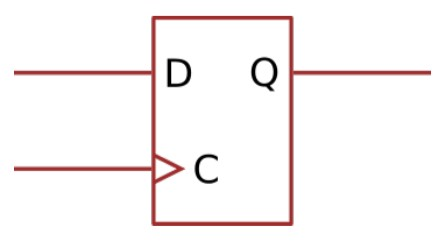
\includegraphics[scale=0.25]{flipflop}
\end{center}
Der Anschluss D ist der Dateneingang, Q der Datenausgang und C ist der Clock-Eingang.
Bei jeder ansteigenden Flanke am Clock-Eingang C übernimmt der Flip-Flop den Zustand vom Eingang D und hält ihn am Ausgang Q fest, bis der Clock eine erneute ansteigende Flanke erhält.

Ein einzelner Flip-Flop kann zwei Zustände speichern, während zwei Flip-Flops vier Zustände speichern können.
Daraus lässt sich ableiten, dass $n$ Flip-Flops $2^n$ Zustände annehmen können.

\subsection{Finite State Machine}\label{subsec:finite-state-machine}

Eine Finite-State-Machine ist eine Schaltung, die Speicher enthält und eine endliche Anzahl von Zustände annehmen kann (daher der Name).
Das Ausgangssignal ist abhängig vom aktuellen Zustand und den Eingangssignalen.
\begin{center}
    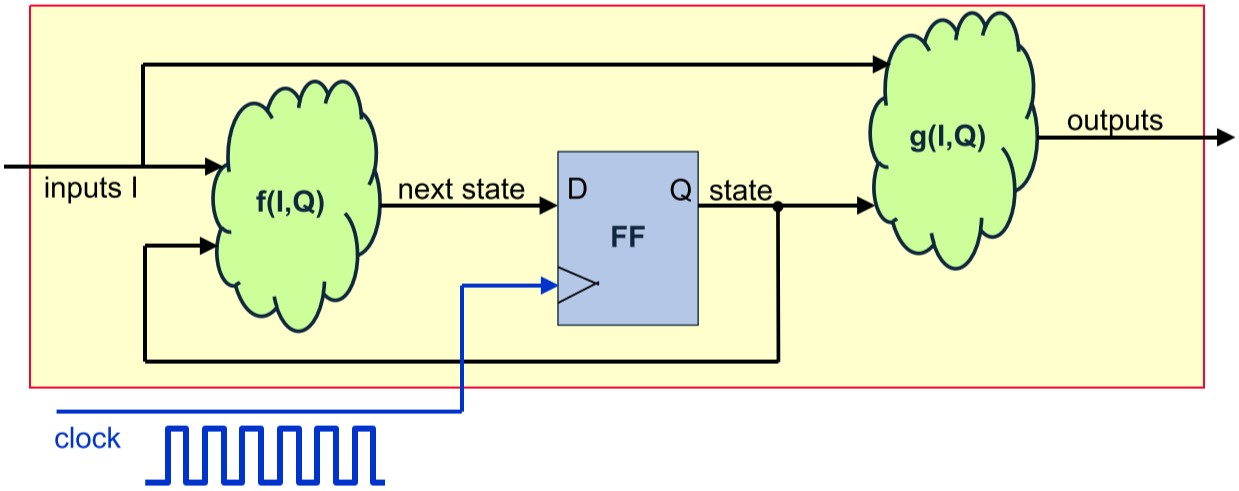
\includegraphics[scale=0.3]{finite-state-machine}
\end{center}
Der $FF$-Block stellt einen Flip-Flop dar und entspricht dem Zustand des Automaten.
Bei jedem Takt-Signal (Clock) wird der Speicher neu geladen.

\subsection{Shiftregister}\label{subsec:register}

Ein Shiftregister (dt.\ Schieberegister) ist eine Schaltung, die mehrere in Reihe geschaltete Flip-Flops enthält.
Bei jedem Signaltakt verschiebt sich der Speicherinhalt der Flip-Flops um eine Position weiter.
Die Anzahl der im Register vorhandenen Speicherplätze ist konstant.
Schieberegister arbeiten nach dem FIFO-Prinzip (First In - First Out), d.h.\ das zuerst eingespeicherte Bit verlässt den Speicher wieder zuerst.
\begin{center}
    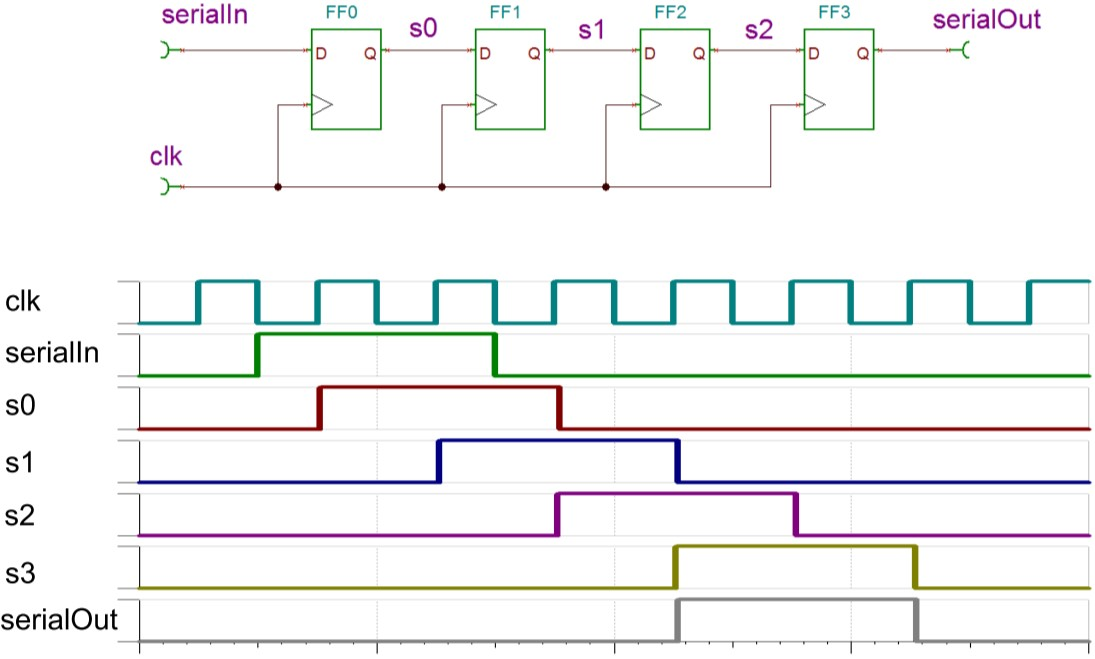
\includegraphics[scale=0.3]{shiftregister-timing-diagram}
\end{center}

    \section{Zahlensysteme}\label{sec:zahlensysteme}

\begin{comment}
    \subsection{Vergleich}\label{subsec:vergleich}
    \begin{center}
        \begin{tabular}{|c|c|c|}
            \hline
            10-er System & 2-er System & 16-er System \\
            \hline
            \hline
            0            & 0000        & 0            \\
            \hline
            1            & 0001        & 1            \\
            \hline
            2            & 0010        & 2            \\
            \hline
            3            & 0011        & 3            \\
            \hline
            4            & 0100        & 4            \\
            \hline
            5            & 0101        & 5            \\
            \hline
            6            & 0110        & 6            \\
            \hline
            7            & 0111        & 7            \\
            \hline
            8            & 1000        & 8            \\
            \hline
            9            & 1001        & 9            \\
            \hline
            10           & 1010        & A            \\
            \hline
            11           & 1011        & B            \\
            \hline
            12           & 1100        & C            \\
            \hline
            13           & 1101        & D            \\
            \hline
            14           & 1110        & E            \\
            \hline
            15           & 1111        & F            \\
            \hline
        \end{tabular}
    \end{center}
\end{comment}

\subsection{Umrechnung}\label{subsec:umrechnung}

\textbf{10-er ins 16-er System:} In einem Beispiel wollen 100 ins 16-er System umwandeln
\begin{align*}
    100_d \div 16 &= 6 \text{ Rest } 4 \\
    6 \div 16 &= 0 \text{ Rest } 6
\end{align*}
Es folgt: $100_d = 64_h$

Überprüfung: $64_h = 6 \cdot 16_d^1 + 4 \cdot 16_d^0 = 100_d$

\textbf{10-er ins 2-er System:} In diesem Beispiel wollen sehen, wie Zahlen mit Kommastellen umgewandelt werden.
Wir wählen hierzu den Wert $26.6875_d$, den wir zu Beginn zerlegen: $26.6875_d = 26_d + 0.6875_d$.

Zuerst wandeln wir den ganzzahligen Teil um:
\begin{align*}
    26_d \div 2 &= 13 \text{ Rest } 0 \\
    13_d \div 2 &= 6 \text{ Rest } 1 \\
    6_d \div 2 &= 3 \text{ Rest } 0 \\
    3_d \div 2 &= 1 \text{ Rest } 1 \\
    1_d \div 2 &= 0 \text{ Rest } 1
\end{align*}
Wir erhalten also: $26_d = 11010_b$

Wir wandeln nun den Bruchteil mithilfe des Horner-Schemas um:
\begin{align*}
    0.6875_d \cdot 2 &= 0.3750 + 1 \\
    0.3750_d \cdot 2 &= 0.7500 + 0 \\
    0.7500_d \cdot 2 &= 0.5000 + 1 \\
    0.5000_d \cdot 2 &= 0.0000 + 1
\end{align*}
Hier erhalten wir also: $0.6875_d = 0.1011_b$

Es folgt das Resultat: $26.6875_d = 11010.1011_b$

\subsection{Negative Zahlen}\label{subsec:negative-zahlen}

Wir haben die Zahl $-3.125_d$, die wir im 2-er System darstellen wollen.
Zu Beginn wandeln wir die Zahl ins 2-er System um: $3.125_d = 110.001_b$.
Anschliessend invertieren wir alle Bits und addieren 1 dazu:
\begin{center}
    \begin{tabular}{cccc}
        Ursprüngliche Zahl & $\dots 0 \ 0 \ 1 \ 1 \ 0. \ 0 \ 0 \ 1$ & b \\
        \hline
        1-er Komplement    & $\dots 1 \ 1 \ 0 \ 0 \ 1. \ 1 \ 1 \ 0$ & b \\
        \hline
        2-er Komplement    & $\dots 1 \ 1 \ 0 \ 0 \ 1. \ 1 \ 1 \ 1$ & b
    \end{tabular}
\end{center}
Diese Technik heisst 2-er Komplement und wird genutzt, um das Vorzeichen von Binärzahlen zu wechseln.

\subsection{Endliche Zahlen}\label{subsec:endliche-zahlen}

\begin{center}
    \begin{tabular}{|c|c|c|c|}
        \hline
        Register & Bezeichnung & \multicolumn{2}{c|}{Maximal darstellbare Zahl} \\
        \hline
        \hline
        4 Bit   & Nibble ($\frac{1}{2}$ Byte) & $0 \dots 15_d$                 & $-8 \dots \text{+}7$                                   \\
        \hline
        8 Bit   & Byte                        & $0 \dots 255_d$                & $-128 \dots \text{+}127$                               \\
        \hline
        16 Bit  & Word                        & $0 \dots 65'535_d$             & $-32'768 \dots \text{+}32'767$                         \\
        \hline
        32 Bit  & Double Word                 & $0 \dots 4.29_d \cdot 10^9$    & $-2.15 \cdot 10^9 \dots \text{+}2.15 \cdot 10^9$       \\
        \hline
        64 Bit  & Long Word                   & $0 \dots 1.84_d \cdot 10^{19}$ & $-9.22 \cdot 10^{18} \dots \text{+}9.22 \cdot 10^{18}$ \\
        \hline
        128 Bit & Double Long Word            & $0 \dots 3.40_d \cdot 10^{38}$ & $-1.70 \cdot 10^{38} \dots \text{+}1.70 \cdot 10^{38}$ \\
        \hline
    \end{tabular}
\end{center}

    \section{Informationstheorie}\label{sec:informationstheorie}

\subsection{Information}\label{subsec:information}

\begin{definition}{Datenquelle}
    \begin{itemize}
        \item \textbf{DMS} (Discrete Memoryless Source): Diese Quelle liefert einzelne Nachrichten, die unabhängig voneinander und gleichverteilt sind (\emph{discrete}), und sie merkt sich die vergangene Nachricht nicht (\emph{memoryless}).
        Folglich sind aufeinanderfolgende Symbole (statistisch) voneinander unabhängig.
        \item \textbf{BMS} (Binary Memoryless Source): Bei dieser Quelle handelt es sich um eine DMS, die aber nur zwei verschiedene Ereignisse erzeugt.
    \end{itemize}
\end{definition}

\begin{definition}{Wahrscheinlichkeit}
    Für die Wahrscheinlichkeit $P(x_n)$ eines Ereignisses $x_n$ gilt: \[P(x_n) = \frac{\text{Anzahl der Ergebnisse, bei denen das Ereignis $x_n$ eintritt}}{\text{Anzahl aller mögliche Ergebnisse}} = \frac{|x_n|}{|\Omega|}.\]
\end{definition}

\begin{definition}{Informationsgehalt}
    Der Informationsgehalt $I(X)$ beim Auftreten von $X_k = x_n$ ist definiert als: \[I = \log_2 \frac{1}{P(x_n)} = -\log_2 P(x_n). \quad \text{[\emph{Bit}]}\]
    Die Masseinheit der Information gibt an, wie viele Bits für das Codieren des betreffenden Symbols notwendig wären, wenn alle Symbole dieselbe Auftretenswahrscheinlichkeit hätten.
\end{definition}

\subsection{Entropie}\label{subsec:entropie}

\begin{definition}{Definition}
    Eine Datenquelle hat eine tiefe Entropie, wenn das nächste Ereignis (Symbol) mit hoher Wahrscheinlichkeit korrekt vorhersagbar ist.
    Wenn diese Wahrscheinlichkeit klein ist, dann ist die Entropie hoch.
\end{definition}

\begin{definition}{Entropie von Quellen}
    Die Entropie $H(X)$ einer Quelle $X$, die statistisch unabhängige Symbole (Ereignisse) $x_n$ liefert, ist definiert als der Erwartungswert der Information $I(x_n)$ dieser Symbole: \[H(X) = \sum_{n=0}^{N-1} P(x_n) \cdot I(x_n)\]
    Die vollständige Formel ist also: \[H(X) = \sum_{n=0}^{N-1} P(x_n) \cdot \log_2 \frac{1}{P(x_n)} = -\sum_{n=0}^{N-1} P(x_n) \cdot \log_2 P(x_n). \quad \text{[\emph{Bit/Symbol}]}\]
\end{definition}

\begin{definition}{Entropie eines BMS (Binäre Entropiefunktion)}
    \[H_b = p \cdot \log_2 \frac{1}{p} + (1-p) \cdot \log_2 \frac{1}{1-p} \quad \text{[\emph{Bit/Symbol}]}\]
\end{definition}

    \section{Quellencodierung}\label{sec:quellencodierung}

\subsection{Quellencodierungstheorem}\label{subsec:quellencodierungstheorem}

\begin{definition}{Codewortl\"ange}
    Sei $l_n$ die Codewortlängen.
    Die mittlere Codewortlänge $L$ einer Quelle, welche die Symbole $x_n$ mit $n = 0,\dots,N-1$ liefert, wird berechnet durch: \[L = \sum_{n=0}^{N-1} P(x_n) \cdot l_n \quad \text{[\emph{Bits/Symbol}]}\]
\end{definition}

\begin{definition}{Redundanz}
    Die Redundanz $R$ eines Codes wird berechnet durch: \[R = L - H \quad \text{[\emph{Bit/Symbol}]}\]
    Bei $R > 0$ umfasst der Code mehr Bits als nötig.
    Bei $R < 0$ reicht die Anzahl Bits pro Codewort nicht aus und Information geht verloren.
\end{definition}

\begin{definition}{Theorem zur Quellencodierung}
    Solange die Redundanz $R$ eines Codes grösser als $0$ ist, kann noch verlustfrei komprimiert werden.
    Falls $R \leq 0$, so kann nur noch verlustbehaftet komprimiert werden.
\end{definition}

\begin{subbox}{}
    \textbf{Kompressionsrate}: $R = \frac{\text{Codierte Bits}}{\text{Originale Bits}}$\\
    \textbf{Präfixfreie Codes:} Kein Code bildet den Anfang eines anderen Codes.
\end{subbox}

\subsection{Lauflängencodierung}\label{subsec:lauflangencodierung}

Die Lauflängencodierung (engl.\ Run Length Encoding, RLE) ist eine lose Sammlung von ähnlichen Methoden zur Komprimierung von Sequenzen (engl.\ Runs) identischer Symbole.
Die zentrale Idee ist, dass Ketten von identischen Zeichen zusammengefasst werden.

\textbf{Beispiel:} Die Sequenz \texttt{aaabbbcc} kann durch die Sequenz \texttt{3a3b2c} komprimiert werden.

\subsection{Huffman-Codes}\label{subsec:huffman-codes}

\begin{subbox}{Rezept Huffman-Verfahren}
    \begin{itemize}
        \item Ordne alle Symbole nach aufsteigenden Wahrscheinlichkeiten an, sie stellen die Blätter des Huffman-Baums dar.
        Gibt es Symbole mit gleicher Wahrscheinlichkeit, so spielt die Reihenfolge unter ihnen keine Rolle.
        \item Notiere unter jedem Symbol seine Wahrscheinlichkeit.
        \item Schliesse die beiden Blätter mit der kleinsten Wahrscheinlichkeit zu einem Knoten zusammen.
        Ordne dem Knoten die Summe der Wahrscheinlichkeiten der beiden Blätter zu.
        \item Wiederhole Schritt 3 so lange, bis nur noch der Stamm des Baums übrig ist.
        \item Nun wird festgelegt, ob bei jedem Knoten der linke Zweig eine 0 oder eine 1 erhält.
        Der rechte Zweig erhält dann das Komplement.
        Frei wählbar, aber muss überall einheitlich sein.
        \item Nun werden auf dem Pfad zu jedem Blatt die Nullen und Einsen ausgelesen und von links nach rechts nebeneinander geschrieben.
        Dies sind die Huffman-Codeworte.
    \end{itemize}
\end{subbox}

\subsection{LZ77}\label{subsec:lz77}

Beim LZ77-Verfahren verwenden wir Token, die aus drei Teilen aufgebaut sind: \textbf{Offset} beschreibt die Distanz zwischen dem ersten Zeichen im Vorschau und dem Ort der besten Übereinstimmung im Such-Buffer.
Die \textbf{Länge} gibt an, wie viele Zeichen übereinstimmen.
Schlussendlich wird ein \textbf{Zeichen} zusätzlich angehängt.
\begin{center}
    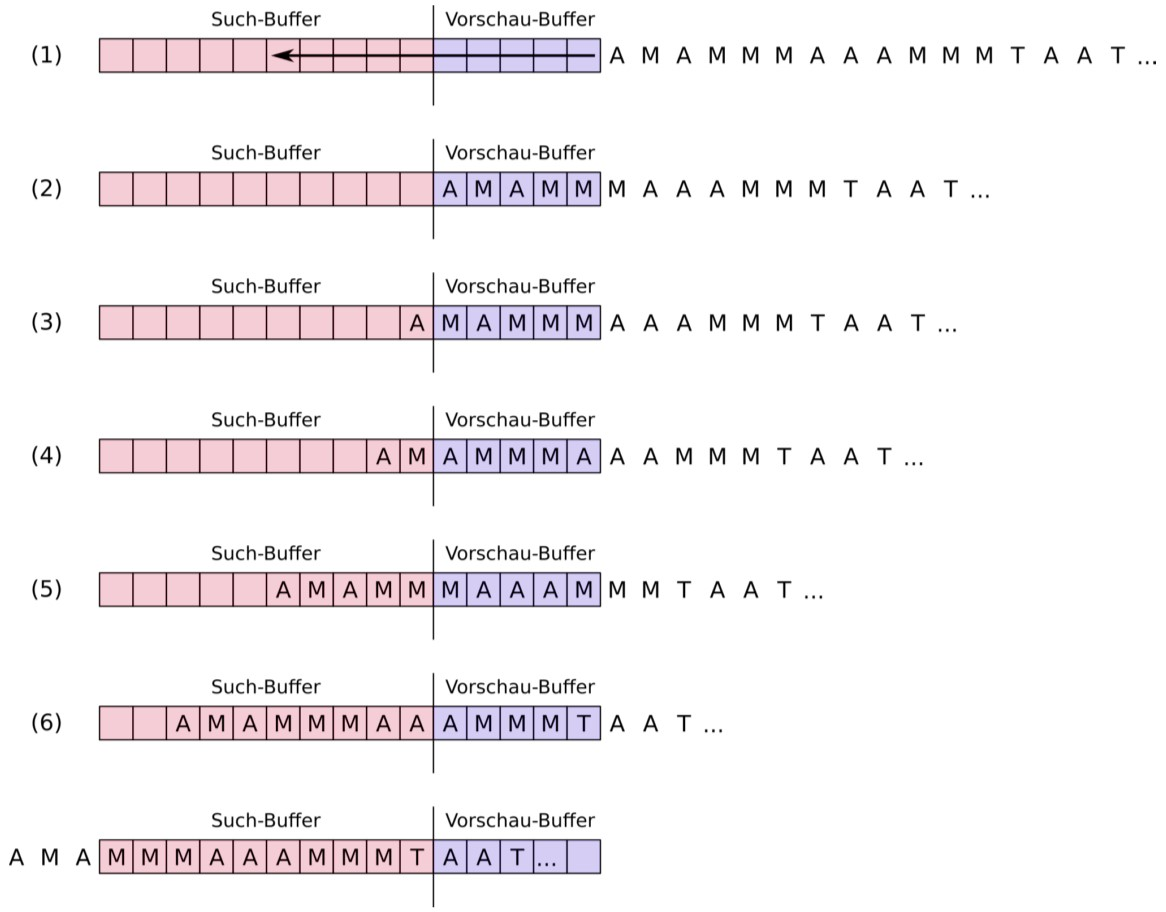
\includegraphics[scale=0.45]{LZ77-example}
\end{center}
Nach dem Ausführen des Verfahrens haben wir die Token (0,0,A), (0,0,M), (2,2,M), (4,2,A) und (6,4,T).

\subsection{LZW}\label{subsec:lzw}
\begin{center}
    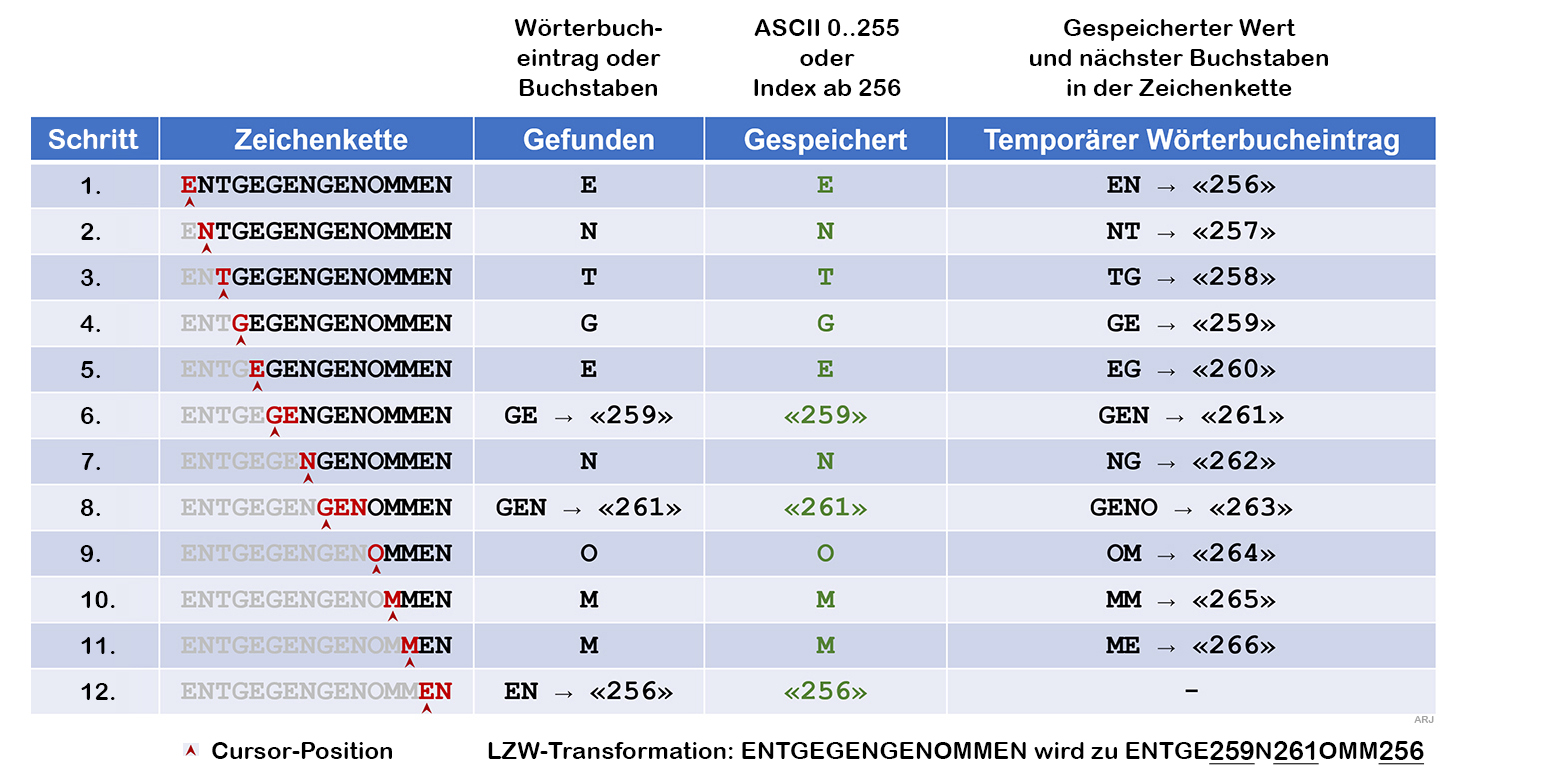
\includegraphics[scale=0.35]{LZW-example}
\end{center}

    \section{JPEG}\label{sec:jpeg}

\subsection{JPEG-Kompression}\label{subsec:jpeg-kompression}

\begin{enumerate}[label={\bfseries Schritt \arabic*:}, wide=0pt]
    \item \textbf{Transformation Farbbilder RGB $\Rightarrow$ Luminanz / Chrominanz}

    Das Auge ist empfindlicher auf kleine Helligkeitsunterschiede als auf kleine Farbunterschiede, d.h.\ die Farbinformation kann höher komprimiert werden, ohne dass man es merkt (Irrelevanz).

    \item \textbf{Downsampling der beiden Chrominanz-Komponenten}

    \begin{itemize}
        \item 2:1 horizontal und vertikal (2h2v oder 4:2:0) \\
        $\Rightarrow$ Bildgrösse: $1/3 + (2/3) \cdot (1/4) = 1/2$
        \item 2:1 horizontal und 1:1 vertikal (2h1v oder 4:2:2) \\
        $\Rightarrow$ Bildgrösse: $1/3 + (2/3) \cdot (1/2) = 2/3$
    \end{itemize}

    \item \textbf{Pixel-Gruppierung der Farbkomponenten in 8x8 Blöcke}

    In diesem Schritt werden die horizontalen und vertikalen Korrelation ausgenutzt.
    Blöcke werden separat komprimiert, was die Schwachstelle von JPEG ist.

    \item \textbf{Diskrete Cosinustransformation (8x8 DCT)}

    Transformation in den Frequenzbereich, was die Vorbereitung für die Datenkompression ist.
    DC und 3--4 tieffrequente AC-Werte enthalten die ``Bildinformation''.

    \item \textbf{Individuelle Quantisierung einzelner Frequenzkomponenten}

    Im Prinzip werden die Frequenzkomponenten mit viel bzw.\ wenig Bildinformation fein bzw.\ grob quantisiert.

    \item \textbf{Entropiecodierung der quantisierten Frequenzkomponenten}

    Dieser Schritt verläuft verlustlos und ist eine Kombination von RLE und Huffman-Encoding.

    \item \textbf{Hinzufügen von Header und JPEG Parameter}
\end{enumerate}

\begin{definition}{Zweidimensionale DCT}
    \begin{itemize}
        \item \textbf{Forward DCT (JPEG: 8x8)} \[F_{vu} = \frac{1}{4} C_u C_v \sum_{x=0}^{7} \sum_{y=0}^{7} B_{yx} \cos \left( \frac{(2x+1)u\Pi}{16} \right) \cos \left( \frac{(2y+1)v\Pi}{16} \right),\] wobei $C_u,C_v = \frac{1}{\sqrt{2}}$ für $u=0$ oder $v=0$ und $C_u,C_v = 1$ für andere Fälle ($u \neq 0$ und $v \neq 0$).
        \item \textbf{Inverse DCT (JPEG: 8x8)} \[B_{yx} = \frac{1}{4} \sum_{u=0}^{7} \sum_{v=0}^{7} C_u C_v F_{vu} \cos \left( \frac{(2x+1)u\Pi}{16} \right) \cos \left( \frac{(2y+1)v\Pi}{16} \right)\]
    \end{itemize}
\end{definition}
\begin{center}
    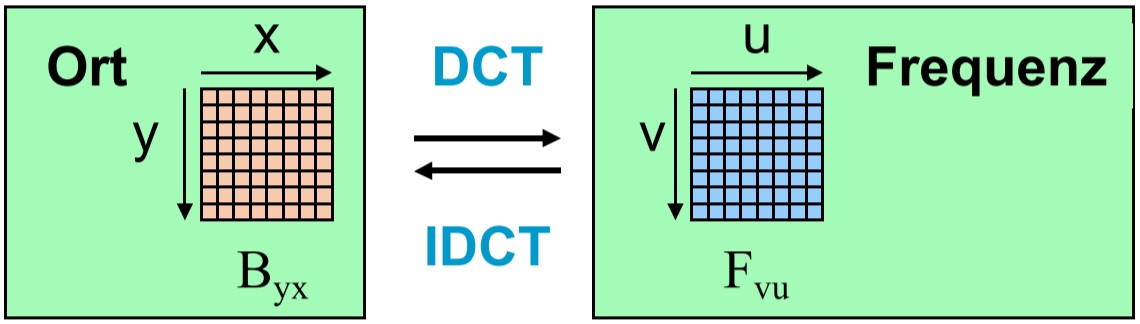
\includegraphics[scale=0.3]{DCT}
\end{center}

\newpage

\subsection{Luminanz und Chrominanz}\label{subsec:luminanz-und-chrominanz}
\begin{multicols}{2}
    \begin{center}
        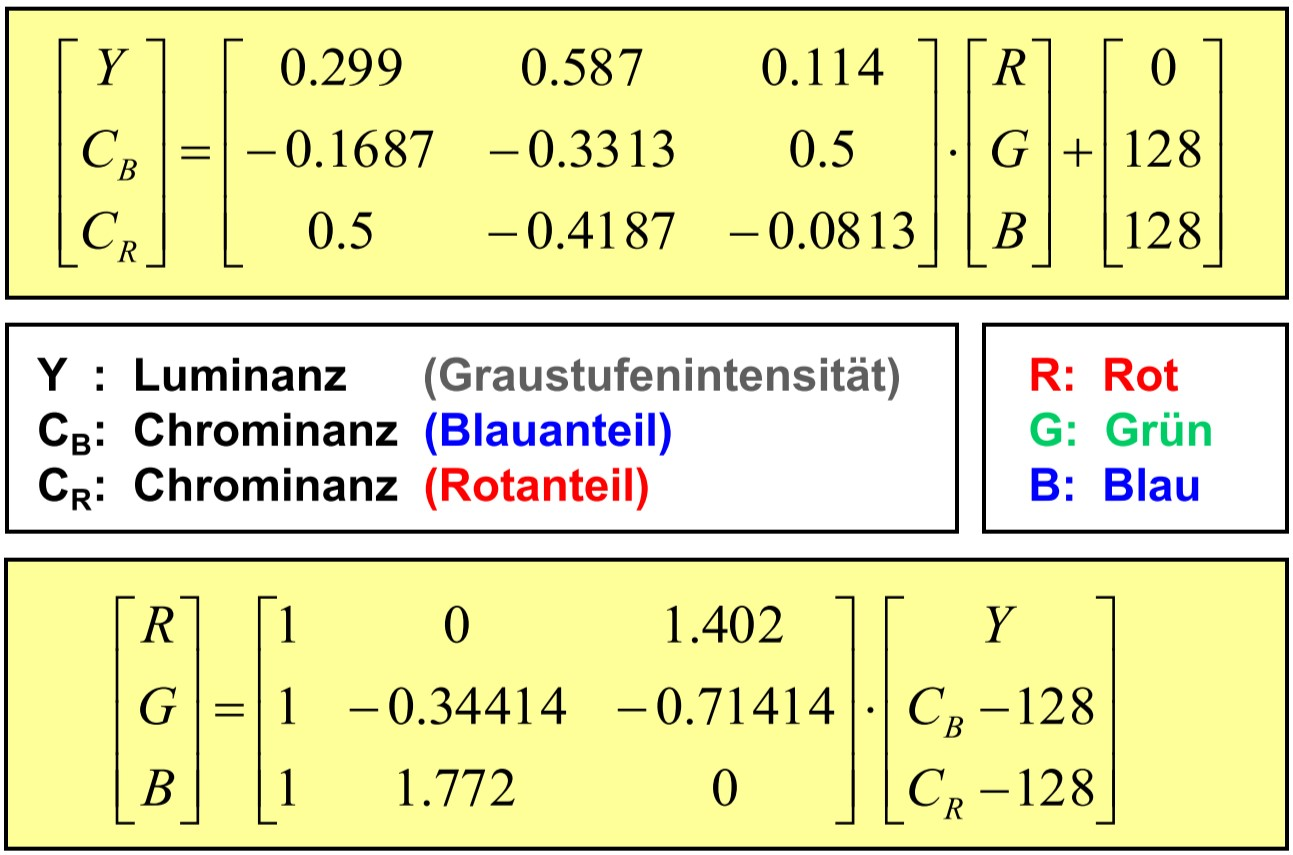
\includegraphics[scale=0.2]{luminanz-chrominanz}
    \end{center}
    \begin{center}
        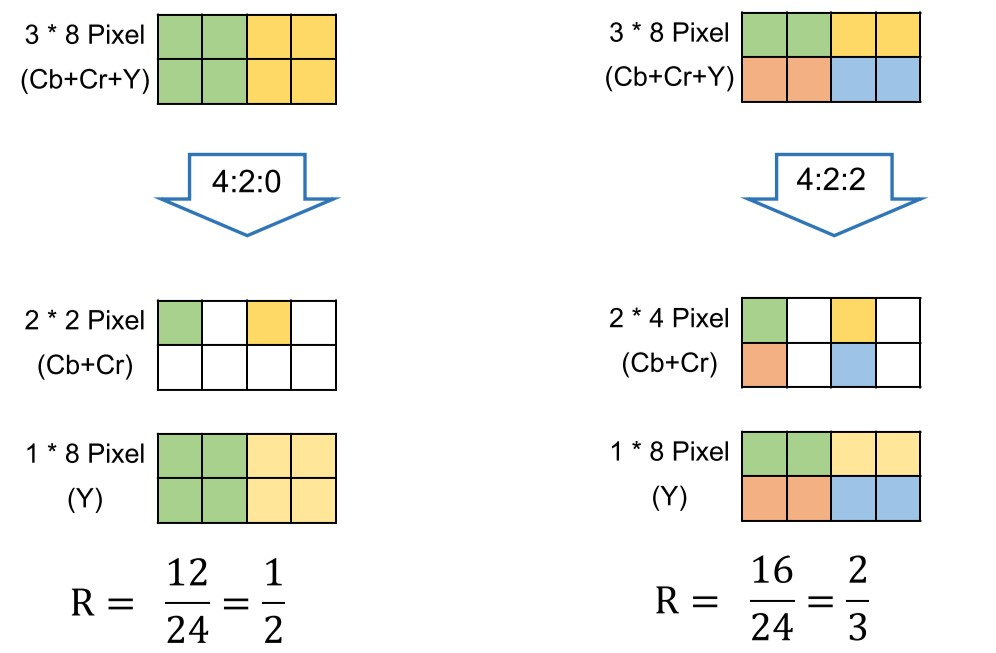
\includegraphics[scale=0.3]{downsampling-example}
    \end{center}
\end{multicols}
\begin{center}
    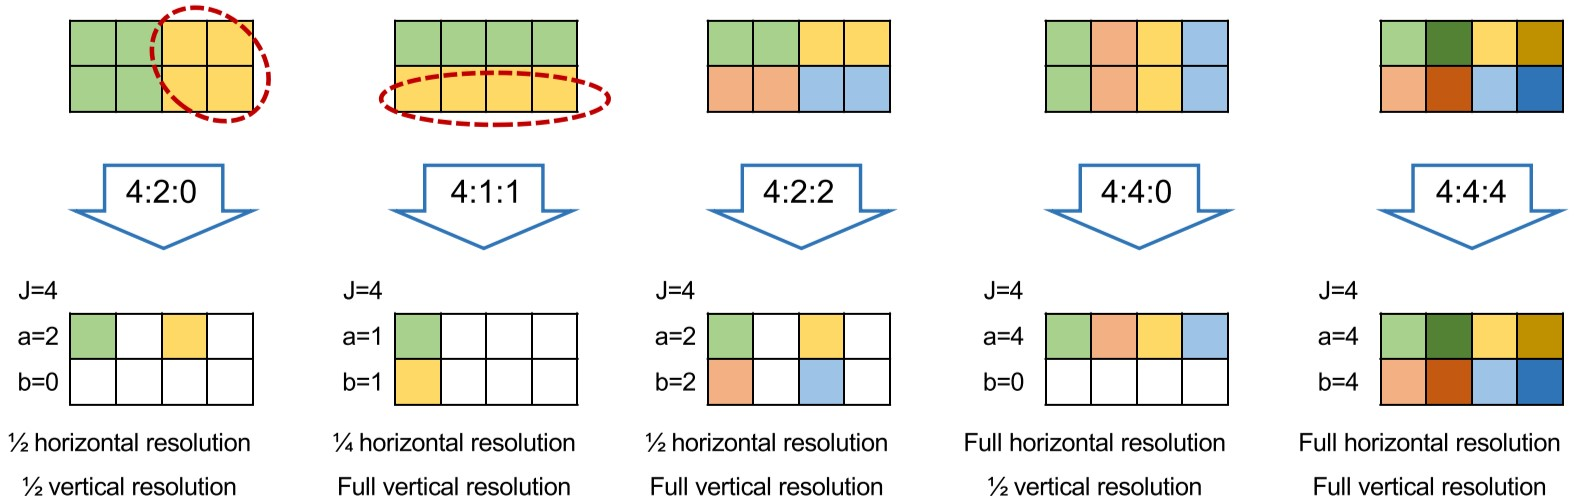
\includegraphics[scale=0.3]{downsampling}
\end{center}

\subsection{JPEG Blockverarbeitung}\label{subsec:jpeg-blockverarbeitung}

\begin{center}
    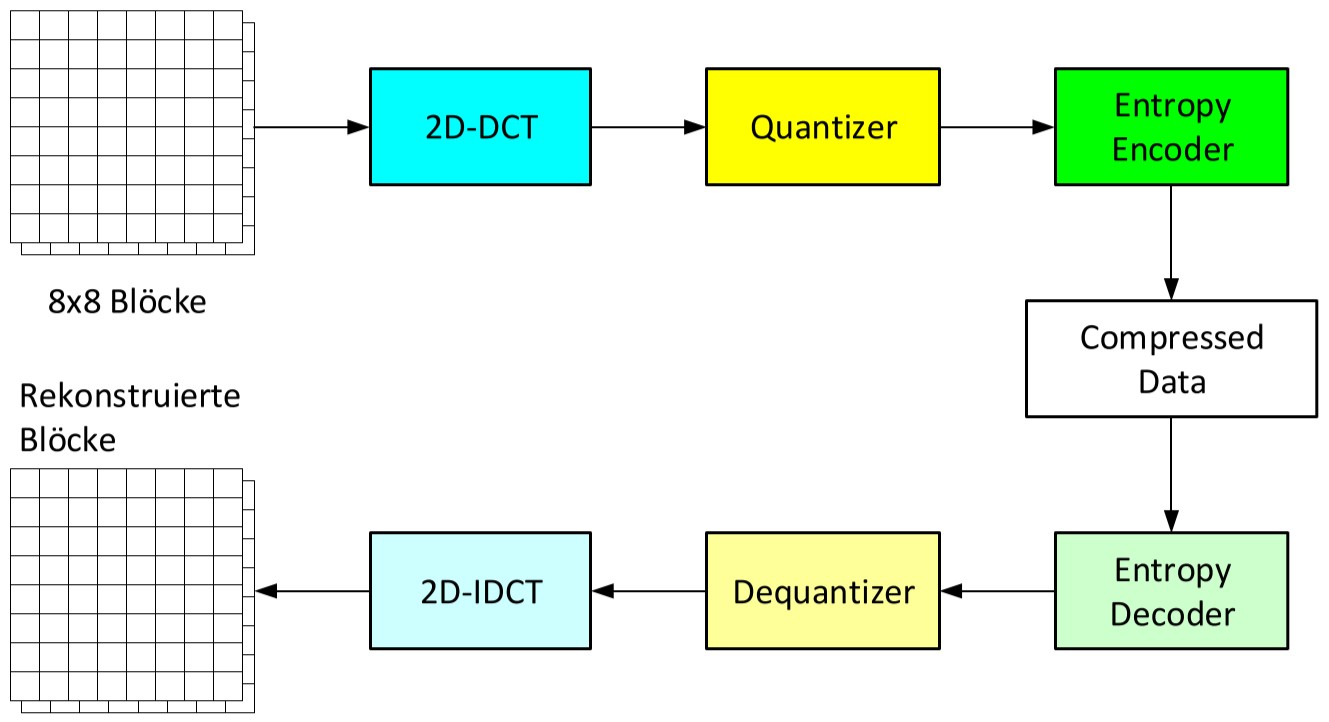
\includegraphics[scale=0.25]{jpeg-blockverarbeitung}
\end{center}

Alle Blöcke zu 8x8 Pixel werden wie folgt weiterverarbeitet:

\begin{itemize}
    \item \emph{Zweidimensionale Diskrete Cosinus-Transformation}: Hierbei werden die Informationen, die als Funktion des Orts vorliegen, in Amplituden von Ortsfrequenzen gewandelt.
    \item \emph{Quantisierer}: Hier wird eine Quantisierung vorgenommen.
    Diese trägt, zusammen mit der Cosinustransformation, wesentlich zur Datenkompression bei, weil bei sehr vielen der insgesamt 64 Werten der Frequenzen nach der Quantisierung der Wert Null übrigbleibt.
    \item \emph{Entropy Encoder}: Die übrigbleibenden relevanten Werten werden nun noch mit einem Entropieverfahren codiert.
    Dies steuert nochmals einen kleinen Beitrag zur gesamten Datenkompression bei.
    Dieser Teil der Kompression ist gänzlich verlustlos, weil Entropieverfahren verlustlos sind.
    \item \emph{Compressed Data}: Die im JPEG-Format komprimierten Daten.
\end{itemize}

    \section{Audio-Codierung}\label{sec:audio-codierung}

\begin{definition}{}
    \textbf{Abtasttheorem von Shannon:} $F_{\text{abtast}} > 2 \cdot f_{\max}$
\end{definition}

\subsection{Pulse Code Modulation (PCM)}\label{subsec:pulse-code-modulation}
\begin{itemize}
    \item \textbf{Filterung:} Zu hohe und zu tiefe Frequenzen werden entfernt, sodass der hörbare Frequenzbereich (etwa 20--20kkHz) übrig bleibt.
    \item \textbf{Abtastung:} Ein zeitkontinuierliches Signal wird in ein zeitdiskretes Signal umgewandelt, indem es in regelmäßigen Abständen registriert wird.
    \item \textbf{Quantisierung:} Die Anzahl Bit, die für die Quantisierung verwendet werden, bestimmt die Anzahl Stufen, welche für die Messung der Amplitude zur Verfügung stehen.
    Die gemessenen Werte werden der nächsten Stufe gerundet zugeordnet.
    Dabei entsteht ein Fehler, der sogenannte \emph{Quantisierungsfehler}.
    \item \textbf{Codierung:} Jedem quantisierten Messwert wird ein Wert von einer bestimmten Bitlänge zugeordnet.
    Aufgrund der Abtastrate entsteht somit ein Bitstrom, der berechnet werden kann mit: \[\text{Anzahl Bit pro Messwert} \cdot \text{Abtastfrequenz}.\]
\end{itemize}

\subsection{Wave File Format}\label{subsec:wave-file-format}

Das \emph{wave}-Dateiformat ist ein Containerformat zur digitalen Speicherung von Audiodaten, wobei der Header Informationen über die Audiodaten enthält.
Wave-Dateien enthalten normalerweise keine komprimierten Audiodaten, sondern die PCM-Rohdaten.
Die Qualität des aufgezeichneten Klangs hängt dann von zwei Werten ab, der Abtastrate (Anzahl Abtastungen pro Zeiteinheit) und der Auflösung der Quantisierung (Bit-Tiefe).

Der File Header besteht aus 44 Byte mit verschiedenen Informationen, wie Format, Anzahl Kanäle, Samples pro Sekunde, Bit pro Sample und Länge der Rohdaten.
Anschliessend folgen die digitalen Audio-Daten, jeweils abwechselnd pro Kanal.

\subsection{Verlustfreie Audio-Codierung}\label{subsec:verlustfreie-audio-codierung}

Im Gegensatz zu verlustbehaftete Audiodatenkompressionsverfahren wie MP3 oder Ogg Vorbis ist die Komprimierung bei FLAC verlustfrei, es gibt also keine Qualitätseinbusse.
Dafür sind die komprimierte Dateien aber auch um ein Vielfaches grösser.

\subsection{Verlustbehaftete Audio-Codierung}\label{subsec:verlustbehaftete-audio-codierung}

\begin{definition}{Schalldruckpegel}
    Um verlustbehaftete Codierung durchführen zu können, braucht es den \emph{Schalldruckpegel}, der die Stärke eines Schallereignisses beschreibt und folgendermassen berechnet wird:
    \[L_P = 10 \log_{10} \left( \frac{\tilde{p}^2}{p_0^2} \right)) \ \text{dB} = 20 \log_{10} \left( \frac{\tilde{p}}{p_0} \right) \ \text{dB},\] wobei $\tilde{p}$ der effektive Schalldruck in Pa ist und $p_0$ der Schalldruckpegel bei einer Schallstärke von 1kHz ist (international auf $0.00002$ Pa gesetzt).
\end{definition}
Eine Verdopplung des effektiven Schalldrucks $p$ entspricht einer Zunahme des Schallpegels um rund \textbf{6dB}, weil \[20 \cdot \log_{10}(2) = 6.02 \ \text{dB}\]


    \section{Kanal-Codierung}\label{sec:kanal-codierung}

\subsection{Fehlerkorrektur}\label{subsec:fehlerkorrektur}

\begin{definition}{Kanalcodierungstheorem von Shannon}
    Man kann über einen diskreten gedächtnislosen Kanal (DMC) mit der Coderate $R$ fehlerfrei übertragen, so lange $R$ nicht grösser ist als die Kanalkapazität.
    Möchte man die Restfehlerwahrscheinlichkeit eines Fehlerschutzcodes beliebig klein machen, so muss $R < C$ sein.
    Hierbei ist $C$ die Kanalkapazität in bit/bit (Nutzbare Bits pro Kanalbenutzung) \[C_{\text{BSC}}(\epsilon) = 1 - H_b(\epsilon)\] und $R$ die Coderate in bit/bit (Infobits pro Codebit) \[R = \frac{K}{N},\] wobei $K$ die Länge der Infowörter und $N$ die Länge der Codewörter ist.
    $R$ muss kleiner als $C$ sein, damit alle Informationen in den nutzbaren Bits Platz hat.
\end{definition}

\subsection{Binäre symmetrische Kanäle}\label{subsec:binaere-symmetrische-kanaele}

Bei einem symmetrischen binären Kanal (engl.\ Binary Symmetric Channel, BSC) gilt:
\begin{itemize}
    \item Die Fehlerwahrscheinlichkeit $\epsilon$ ist unabhängig vom Eingangssymbol.
    \item Die Wahrscheinlichkeiten $P(y_m \mid x_n)$ der Übergänge (bei gegebenem $x_n$) sind:
    \begin{center}
        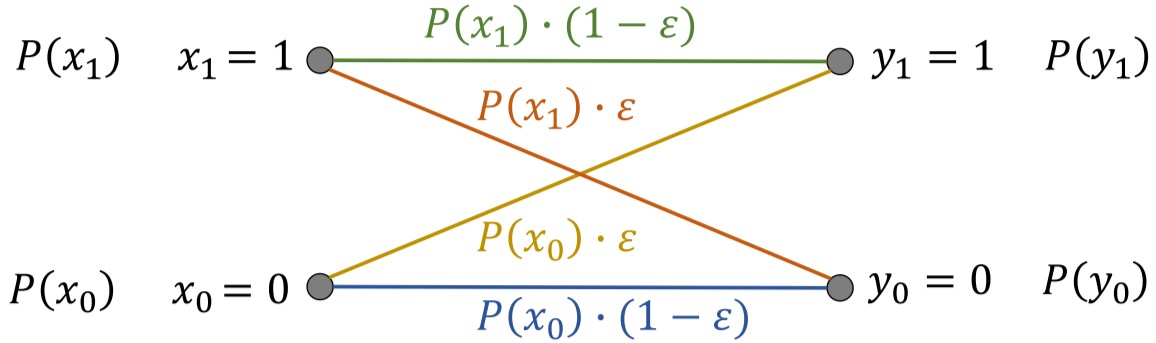
\includegraphics[scale=0.25]{binary-symmetric-channel}
    \end{center}
\end{itemize}

\subsubsection{Bitfehlerwahrscheinlichkeit}

Die \emph{Bitfehlerwahrscheinlichkeit} $\epsilon$ (engl.\ Bit Error Ratio, BER) ist eine Eigenschaft des Kanals, die die Anzahl der fehlerhaften Bits im Verhältnis zur Gesamtzahl der Bits angibt.
Beispiele:
\begin{multicols}{2}
    \begin{itemize}
        \item Alle Bits falsch: BER = 1
        \item Kein Bit falsch: BER = 0
        \item 1 von 2 Bits falsch: BER = 0.5
        \item 1 von 1000 Bits falsch: BER = 0.001
    \end{itemize}
\end{multicols}

\subsubsection{Mehr-Bit-Fehlerwahrscheinlichkeiten}

\begin{definition}{Binomialkoeffizient}
    $\binom{n}{k}$ ist der $k$-te Koeffizient der Potenz des Binoms $(x + y)^n$.
    Es gilt mit $k \leq n$: $\binom{n}{k} = \frac{n!}{k! \cdot (n-k)!}.$
\end{definition}

\begin{definition}{}
    Die Wahrscheinlichkeit $P_{F,N}$, dass in einer Sequenz von $N$ Datenbits \emph{genau $F$ Bitfehler} auftreten, ist gegeben durch \[P_{F,N} = \binom{N}{F} \cdot \epsilon^F \cdot (1 - \epsilon)^{N-F},\] wobei der Binomialkoeffizient die Anzahl der Möglichkeiten angibt, $F$ Fehler in $N$ Bits anzuordnen. $\epsilon^F$ ist die Wahrscheinlichkeit für einen $F$-fachen Bit-Fehler, und $(1 - \epsilon)^{N-F}$ ist die Wahrscheinlichkeit, dass die restlichen $N-F$ Bits alle keinen Fehler haben.
\end{definition}

Für die Wahrscheinlichkeit, dass \emph{maximal $F$ Fehler} bei einer Übertragung von $N$ Bits auftreten, bilden wir die Summe aller Fälle: \[P_{\leq F,N} = \sum_{t=0}^{F} \binom{N}{t} \cdot \epsilon^t \cdot (1 - \epsilon)^{N-t}\]
Oft will man die Restfehlerwahrscheinlichkeit wissen, also die Wahrscheinlichkeit, dass \emph{mehr als $F$ Fehler} bei einer Übertragung von $N$ Bits auftreten: \[P_{\geq F,N} = \sum_{t=F+1}^{N} \binom{N}{t} \cdot \epsilon^t \cdot (1-\epsilon)^{N-t}\]

\subsubsection{Kanalkapazität}

Die maximale Kanalkapazität entspricht dem Maximum der Entropie einer binären Quelle: 1 Bit/Symbol = 1 bit/bit.
Die Störquelle kann ebenfalls als Binary Memoryless Source mit den Wahrscheinlichkeiten $\epsilon$ (Fehler) und $1-\epsilon$ (kein Fehler) betrachtet werden. \[C_{\text{BSC}}(\epsilon) = 1 - H_b(\epsilon) \\
= 1 - \left\{ \epsilon \cdot \log_2 \frac{1}{\epsilon} + (1-\epsilon) \cdot \log_2 \frac{1}{1-\epsilon}\right\}\]

\subsubsection{Hamming-Distanz}

\begin{definition}{Hamming-Distanz}
    Die \emph{Hamming-Distanz} ist die Anzahl der wechselnden Bits von einem gültigen Code zum nächsten gültigen Code
\end{definition}

Die Hamming-Distanz $d$ zwischen den Codewörtern ist nicht per se konstant:
\begin{multicols}{3}
    \begin{itemize}
        \item \texttt{d(00000, 01011) = 3}
        \item \texttt{d(01011, 10101) = 4}
        \item \texttt{d(00000, 10101) = 3}
        \item \texttt{d(01011, 11110) = 3}
        \item \texttt{d(00000, 11110) = 4}
        \item \texttt{d(10101, 11110) = 3}
    \end{itemize}
\end{multicols}

\begin{definition}{Minimale Hamming-Distanz}
    Für eine \emph{sichere} Fehlererkennung ist die minimale Hamming-Distanz $d_{\min}(C)$ eines Codes $C$ relevant: \[d_{\min}(C) = \min \limits_{j \neq k} d_H(c_j, c_k)\]
\end{definition}
Es lassen sich $d_{\min} - 1$ Bit-Fehler pro Codewort sicher erkennen und $\frac{d_{\min} - 1}{2}$ Fehler sicher korrigieren.
\begin{definition}{Hamming-Gewicht}
    Das \emph{Hamming-Gewicht} $w_H(c_j)$ gibt an, wie viele Einsen das Codewort $c_j$ enthält und darf nicht mit der Hamming-Distanz verwechselt werden!
    Sie wird verwendet, um die Hamming-Distanz zweier Codewörter zu bestimmen \[d_H(c_j,c_k) = w_H(c_j \oplus c_k)\]
\end{definition}

\textbf{Beispiele:}
\begin{multicols}{2}
    \begin{itemize}
        \item $w_H(000) = 0$
        \item $w_H(110) = w_H(011) = w_H(101) = 2$
        \item[]
    \end{itemize}
    \begin{itemize}
        \item $d_H(000,110) = w_H(000 \oplus 110) = w_H(110) = 2$
        \item $d_H(110,011) = w_H(110 \oplus 011) = w_H(101) = 2$
        \item $d_H(110,101) = w_H(110 \oplus 101) = w_H(011) = 2$
    \end{itemize}
\end{multicols}

\subsection{Binäre Blockcodes}\label{subsec:binaere-blockcodes}

\begin{itemize}
    \item \textbf{Systematik:} Die Informationsbits erscheinen im Codewort in einem Stück, ohne dass Fehlerschutzbits dazwischen vorhanden sind.
    Systematische Blockcodes sind einfach zu decodieren, da lediglich die Fehlerschutzbits entfernt werden müssen.
    \item \textbf{Linearität:} Bei einem linearen Blockcode ist die bitweise Exor-Verknüpfung von 2 Codewörtern wieder ein gültiges Codewort.
    Jeder lineare Code muss zwingend das Null-Codewort (000) enthalten.
    \item \textbf{Zyklizität:} Die zyklische Verschiebung eines Codeworts gibt wieder ein Codewort.
\end{itemize}

\subsection{Fehlererkennung}\label{subsec:fehlererkennung}

\subsubsection{Parität}

Eine einfache Methode für die Fehlererkennung macht Gebrauch eines \emph{Paritätsbit} (parity bit) über ein Datenbyte.
Hierbei setzen wir \emph{Even Parity}, wenn die Anzahl der Einsen inklusive Parity-Bit gerade ist, und \emph{Odd Parity}, wenn sie ungerade ist.
Beide sind gleichwertig, aber nur Even Parity ist linear.
\begin{center}
    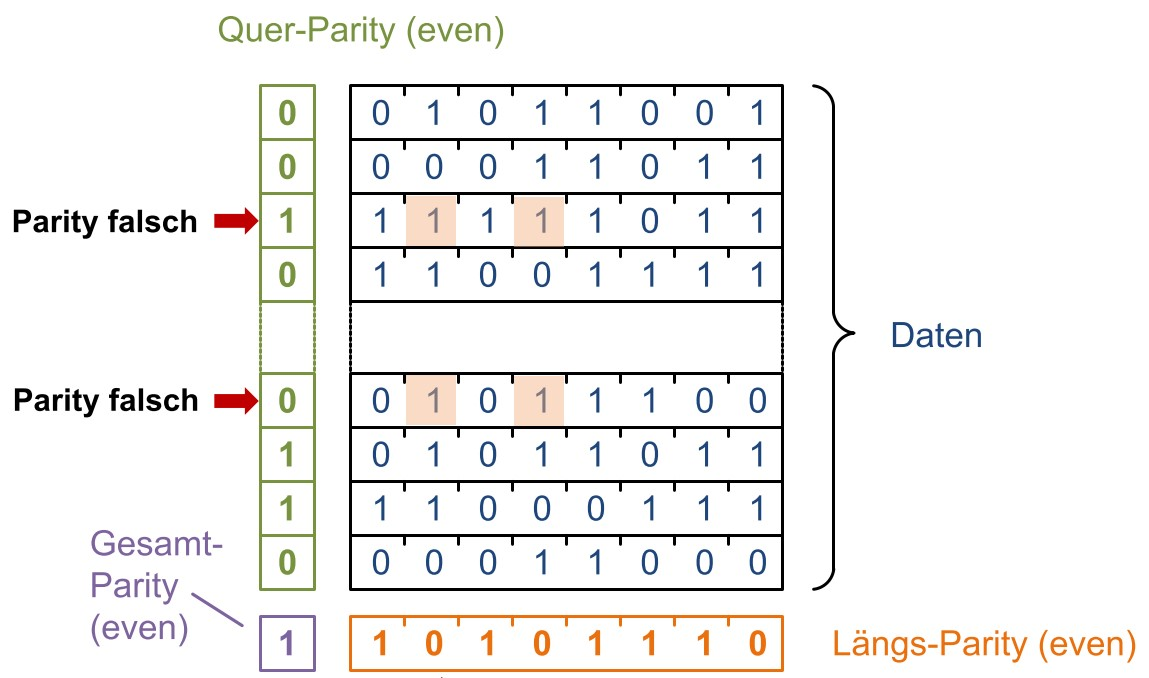
\includegraphics[scale=0.3]{parity}
\end{center}

\subsection{Fehlerkorrigierende Codes}\label{subsec:fehlerkorrigierende-codes}

\subsubsection{Hamming-Codes}

\begin{center}
    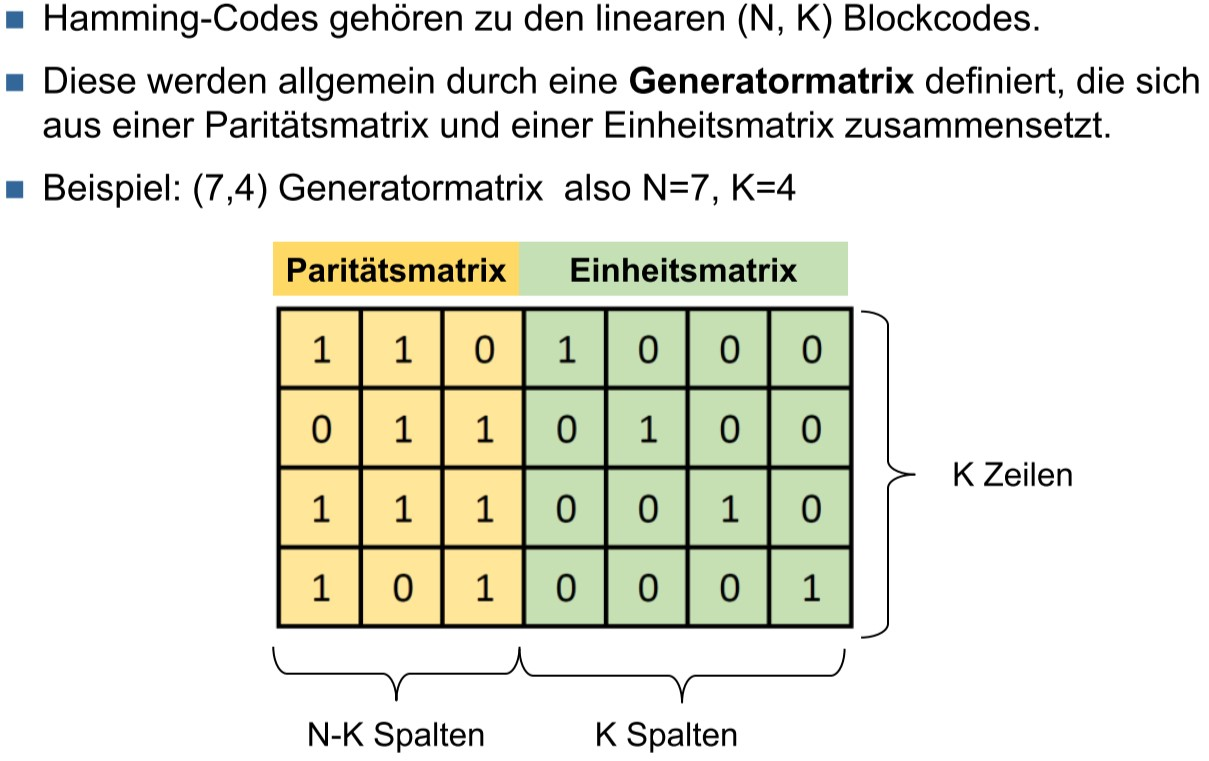
\includegraphics[scale=0.27]{generator-matrix}
    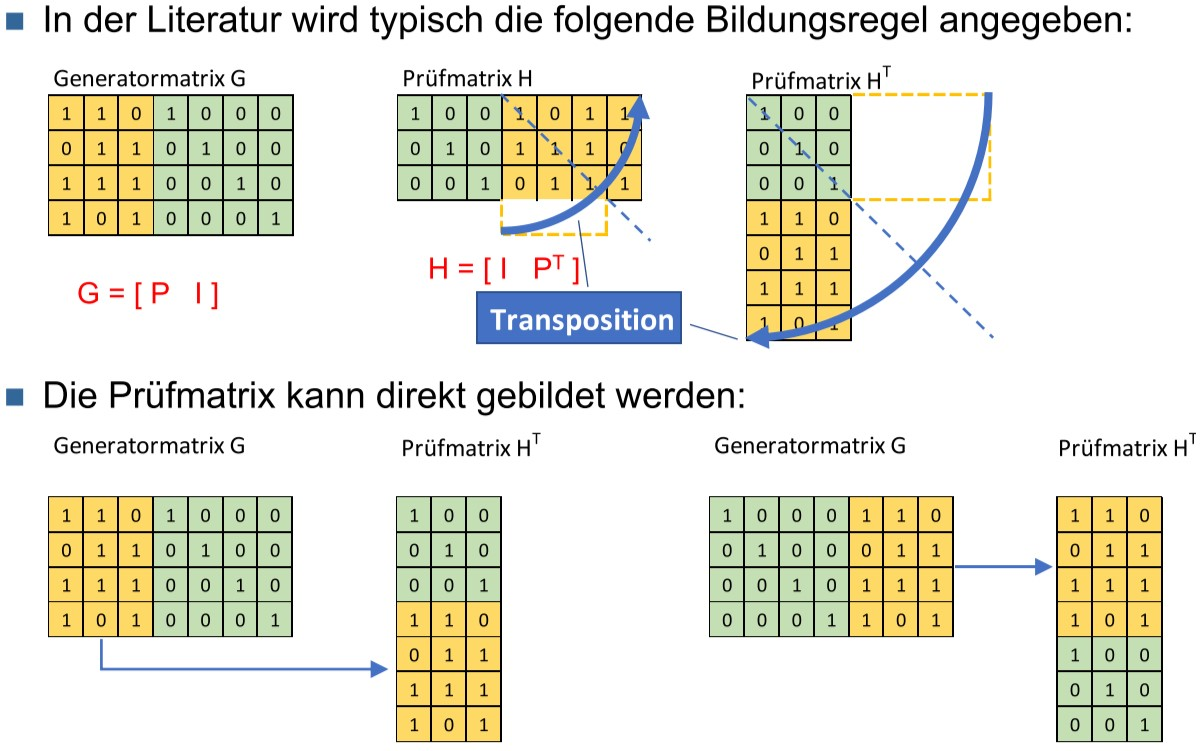
\includegraphics[scale=0.27]{pruef-matrix}
\end{center}

Hamming-Codes sind lineare Blockcodes unterschiedlicher Länge mit einer minimalen Hamming-Distanz von $d_{\min} = 3$.
Diese Codes sind optimal und demnach in der Lage 1-Bit Fehler sicher korrekt zu korrigieren.
2-Bit Fehler lassen sich sicher erkennen.

\subsubsection{Faltungscode}

\begin{definition}{Freie Distanz}
    Bei Faltungscodes spricht man nicht von minimaler Hamming-Distanz, sondern einer \emph{freien Distanz $d_{free}$}.
    Man wählt hierbei den kürzesten Weg von $00$ wieder zu $00$, wobei mind.\ eine 1 im Weg vorhanden sein soll (Zahl unter dem Strich).
\end{definition}

\begin{center}
    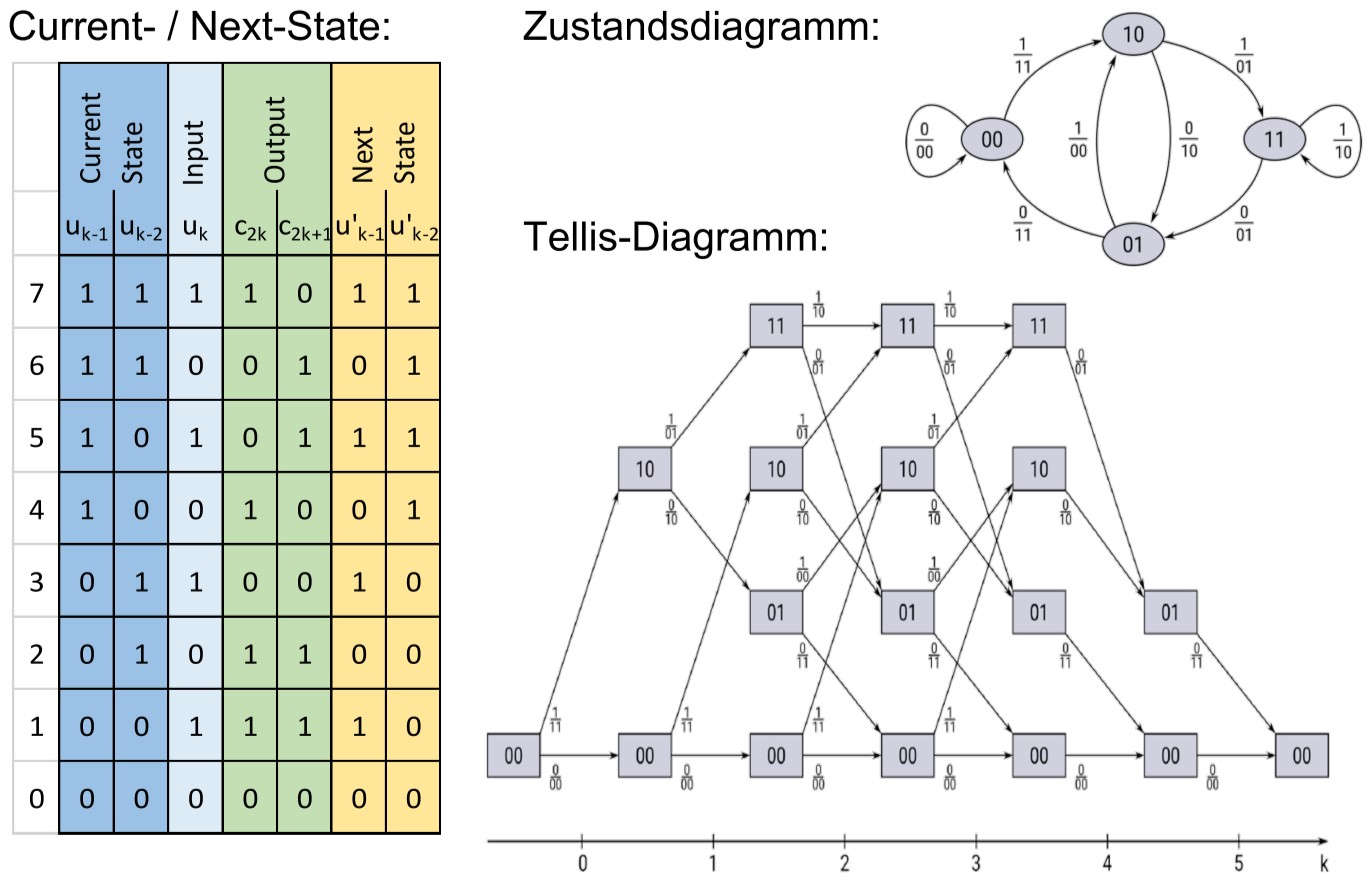
\includegraphics[scale=0.4]{trellis-diagramm}
\end{center}

\begin{center}
    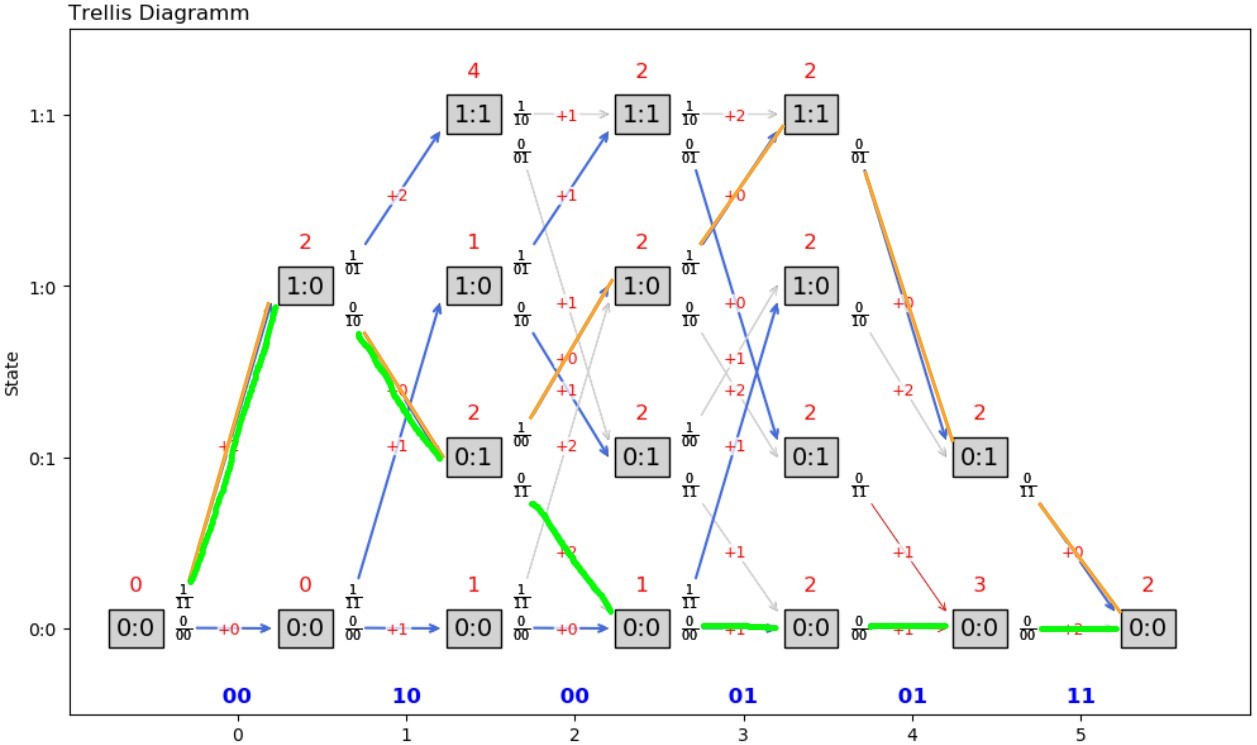
\includegraphics[scale=0.4]{trellis-diagram-example}
\end{center}

    \section{Appendix}\label{sec:appendix}

%\subsection*{Matrizenrechnung}

%\begin{definition}{Matrix}
    Eine \emph{Matrix} ist in der Mathematik eine Anordnung von Werten in Zeilen und Spalten.
    Eine Matrix mit $m$ Zeilen und $n$ Spalten wird als $m \times n$ Matrix bezeichnet und kann wie folgt dargestellt werden:
    \[A = \begin{bmatrix}
              a_{1,1} & a_{1,2} & \dots  & a_{1,n} \\
              \vdots  & \vdots  & \ddots & \vdots  \\
              a_{m,1} & a_{m,2} & \dots  & a_{m,n}
    \end{bmatrix}\]
\end{definition}

\begin{definition}{Matrizenmultiplikation}
    Damit Matrizen multipliziert werden können, muss die Anzahl der Spalten der linken Matrix gleich der Anzahl der Zeilen der rechten Matrix sein.
    Es seien die Matrizen $A \in \R^{m \times n}$ und $B \in \R^{n \times p}$.
    Die Matrix $C = AB$ ist dann die $m \times p$ Matrix, deren Elemente durch die Formel \[c_{ij} = a_{i1}b_{1j} + a_{i2}b_{2j} + \dots + a_{in}b_{nj} = \sum_{k=1}^{n} a_{ik}b_{kj}\] berechnet werden, wobei $i = 1,\dots,m$ und $j = 1,\dots,p$ sind. $AB \neq BA$!
\end{definition}

\textbf{Beispiel:} Es seien die Matrizen
$A =
\begin{bmatrix}
    1 & 2 \\
    3 & 4
\end{bmatrix}$ und $B =
\begin{bmatrix}
    5 & 6 \\
    7 & 8
\end{bmatrix}$.
Dann ist \[AB =
\begin{bmatrix}
    1 \cdot 5 + 2 \cdot 7 & 1 \cdot 6 + 2 \cdot 8 \\
    3 \cdot 5 + 4 \cdot 7 & 3 \cdot 6 + 4 \cdot 8
\end{bmatrix} =
\begin{bmatrix}
    19 & 22 \\
    43 & 50
\end{bmatrix}.\]

\begin{subbox}{Rechenregeln für Matrizen}
    Für die drei Matrizen $A,B,C \in \R^{n \times n}$ gelten folgende Rechenregeln:
    \begin{align*}
        A + B &= B + A &(Kommutativgesetz) \\
        A + (B + C) &= (A + B) + C &(Assoziativgesetz) \\
        C(A + B) &= CA + CB &(Distributivgesetz) \\
        (A + B)C &= AC + BC &(Distributivgesetz) \\
        A(BC) &= (AB)C &(Assoziativgesetz)
    \end{align*}
\end{subbox}

\begin{definition}{Einheitsmatrix}
    Die Einheitsmatrix $I$ ist eine quadratische Matrix, deren Matrixelemente der Hauptdiagonalen alle 1 betragen.
    Alle übrigen Elemente sind 0.
    Beispiele: $I_2 = \begin{bmatrix}
                           1 0 \\
                           0 1
    \end{bmatrix} \quad \quad I_3 = \begin{bmatrix}
                                        1 0 0 \\
                                        0 1 0 \\
                                        0 0 1
    \end{bmatrix}$
\end{definition}

\begin{definition}{Inverse Matrix}
    Eine quadratische Matrix $A$ ist invertierbar, falls eine Matrix $A^{-1}$ existiert, sodass $AA^{-1} = A^{-1}A = I$
\end{definition}

\begin{definition}{Transponierte einer Matrix}
    Beim Transponieren einer Matrix $A$ werden die Zeilen von $A$ zu Spalten von $A^T$ und die Spalten von $A$ zu Zeilen von $A^T$.
    Dies entspricht einer Spiegelung der Matrix an der Diagonalen.
\end{definition}

\begin{center}
    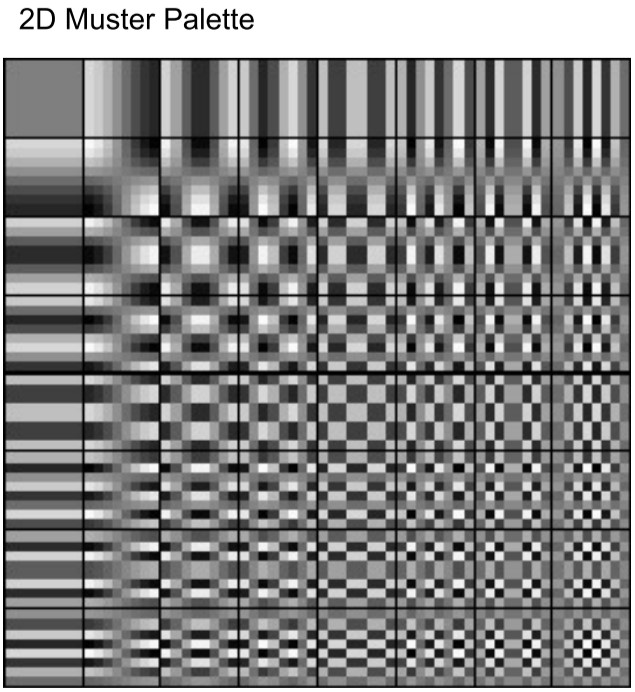
\includegraphics[scale=0.3]{musterpalette}
    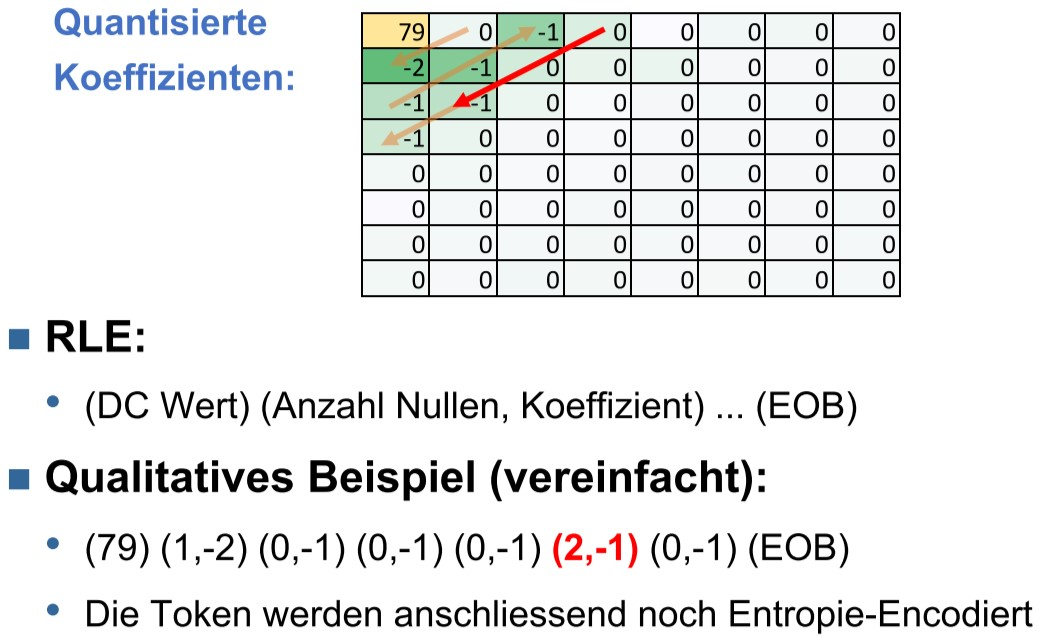
\includegraphics[scale=0.3]{encoding-ac-koefficients}
\end{center}

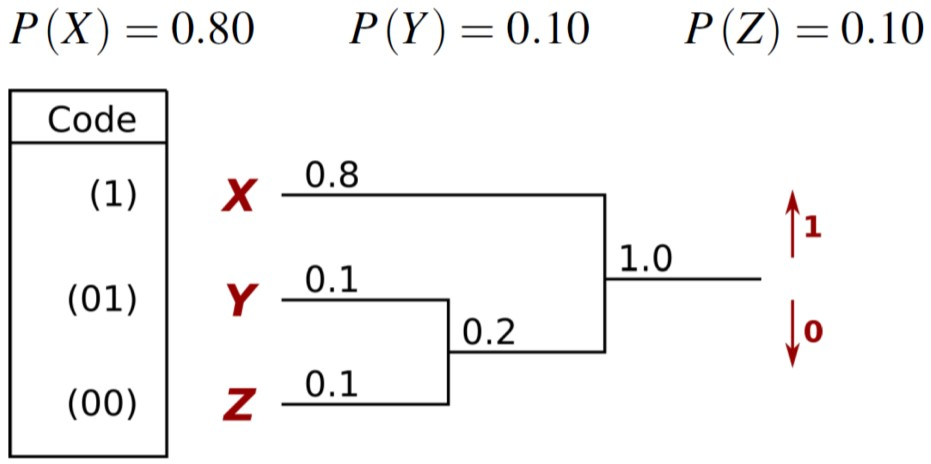
\includegraphics[scale=0.3]{huffman-code}
\end{document}